\documentclass{article}
\usepackage{tikz}
\usetikzlibrary{math}

\begin{document}

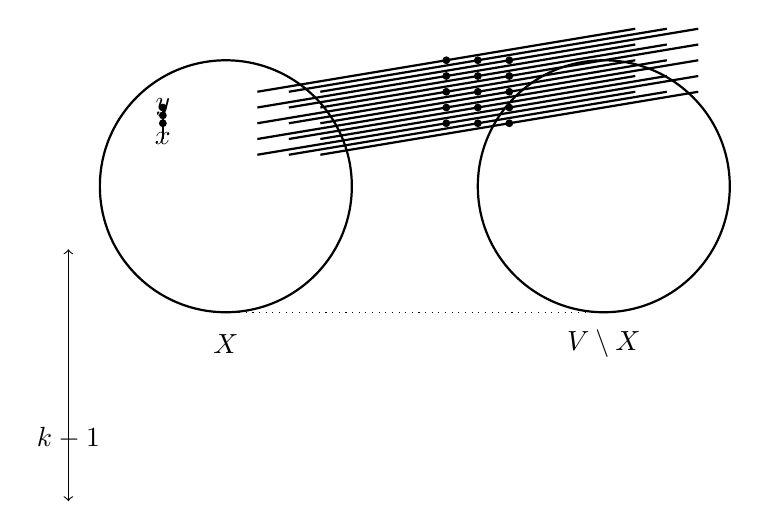
\begin{tikzpicture}[scale=0.8]
    % Draw circles
    \draw[thick] (0,0) circle (2cm);
    \draw[thick] (6,0) circle (2cm);

    % Label sets
    \node at (0,-2.5) {$X$};
    \node at (6,-2.5) {$V \setminus X$};

    % Draw edges from X to V \setminus X
    \foreach \i in {1,...,3}{
        \draw[thick] (0+\i*0.5,0.5) -- node[fill,circle,inner sep=1pt] {} (6+\i*0.5,1.5);
        \draw[thick] (0+\i*0.5,0.75) -- node[fill,circle,inner sep=1pt] {} (6+\i*0.5,1.75);
        \draw[thick] (0+\i*0.5,1.0) -- node[fill,circle,inner sep=1pt] {} (6+\i*0.5,2.0);
        \draw[thick] (0+\i*0.5,1.25) -- node[fill,circle,inner sep=1pt] {} (6+\i*0.5,2.25);
        \draw[thick] (0+\i*0.5,1.5) -- node[fill,circle,inner sep=1pt] {} (6+\i*0.5,2.5);
    }

    % Draw edge xy
    \draw[thick] (-1,1.25) -- node[fill,circle,inner sep=1pt] {} (-1,0.75);
    \draw[thick] (-1,1.25) -- node[fill,circle,inner sep=1pt] {} (-1,1.0);
    \draw[thick] (-1,1.25) -- node[fill,circle,inner sep=1pt] {} (-1,1.25);

    % Label vertices
    \node at (-1,1.25) {$y$};
    \node at (-1,0.75) {$x$};

    % Dotted line
    \draw[dotted] (0,-2) -- (6,-2);

    % Label k-1
    \draw[<-] (-2.5,-1) -- (-2.5,-3);
    \draw[->] (-2.5,-3) -- (-2.5,-5);
    \node at (-2.5,-4) {$k-1$};
\end{tikzpicture}

\end{document}